%! TEX rootmain.tex

\chapter{Drums}

Drums are percussion instruments in which vibrating membranes, often coupled to air volumes and supporting structures, generate sound after impulsive excitation. The perceived pitch, timbre, and decay depend on membrane modes, their coupling to enclosed air and shells, radiation efficiency, and playing technique. The discussion introduces common taxonomies for drums, then focuses on kettledrums, bass drums, snare drums, tom toms, drumhead construction variants, and selected Indian drums.

\section{Types of Percussions and Drums}

A practical distinction separates percussion instruments into pitched and unpitched families.

\begin{itemize}
    \item Pitched percussion instruments convey a strong sense of pitch; typical examples include kettledrums and tabla-type instruments.
    \item Non-pitched percussion instruments emphasize broadband or weakly tonal spectra; typical examples include snare drums, bass drums, tom toms, bongos, congas, and tambourines.
\end{itemize}

\section{Drum Categories}

A second categorization emphasizes how the membrane is coupled to an acoustic load and to structural elements.

\begin{itemize}
    \item Single membrane coupled to an enclosed air cavity, as in kettledrums.
    \item Single membrane mounted on resonant structures, as in congas or djemb\`e-type drums.
    \item Double membrane mounted on a shell, as in bass drums and snare drums.
\end{itemize}

This taxonomy highlights that the same vibrating element (a membrane) can lead to very different radiation and decay behaviors depending on the surrounding air volume and the mechanical boundary conditions set by the frame or shell.

\section{Kettledrums}

\subsection{Instrument Structure and Pitch Control}

Kettledrums (timpani) behave as pitched instruments. Pitch control is achieved through a pedal-operated mechanism that changes the membrane tension, hence shifting modal frequencies. The typical resonator is an approximately hemispherical bowl, often made of copper, and multiple timpani of different sizes are commonly used together in performance. 

\subsection{Harmonic Relationships and the Role of Air Loading}

An ideal membrane exhibits intrinsic inharmonicity, yet kettledrums can produce spectra with more nearly harmonic relationships. Several effects contribute to this partial regularization: 

\begin{itemize}
    \item air loading,
    \item coupling with shell resonances,
    \item air cavity resonances,
    \item membrane bending stiffness,
    \item membrane stiffness to shear.
\end{itemize}

Among these, air loading is the dominant factor in determining the pitched character. Air loading lowers the frequencies of low-order modes and adjusts their ratios toward more harmonic relationships, while the other effects mainly provide finer adjustments and strongly influence decay behavior. Air loading can be described by considering the pressure acting on both sides of the membrane. In a kettledrum, the internal pressure field is shaped by the enclosed cavity and by a small vent-hole placed at the bottom of the bowl, while external radiation provides a second pressure contribution on the outer side of the membrane. A representative comparison of modal ratios illustrates the trend. Modes \((1, 1)\), \((2, 1)\), \((3, 1)\), \((4, 1)\) that would appear at approximately \( 1.00 : 1.34 : 1.66 : 1.98 \) for an ideal membrane are shifted toward ratios close to \( 1.00 : 1.50 : 1.97 : 2.44 \) for a membrane mounted on a kettledrum-like structure. When air loading is present without hinging to a shell, ratios still remain relatively harmonic, around \( 1.00 : 1.47 : 1.91 : 2.36 \), indicating that the shell is less critical for harmonicity than the air loading itself. 

\paragraph{Remark on computed and measured frequencies} For a representative tension value \( T = \SI{3990}{\newton\per\meter} \), calculated modal frequencies can be compared with measured values, and the agreement supports the use of air-loading-based models as a primary explanation of timpani pitch behavior.

\subsection{Excitation, Spectrum Over Time, and Perceived Tone}

The standard striking position is approximately one quarter of the membrane radius inward from the edge. The striking position strongly influences the spectral balance: hitting at the center tends to produce a duller sound with reduced harmonic content, while off-center strikes excite a different mix of modes. Different partials exhibit different decay rates. Axisymmetric \((0, 1)\), \((0, 2)\), \((0, 3)\) modes damp out relatively quickly, whereas modes such as \((1, 1)\), \((2, 1)\), \((3, 1)\), \((4, 1)\) can persist longer and are excited by both central and standard strikes. The \((1, 1)\) mode is typically the longest-lasting and becomes central in determining the perceived tone. In this context, psychoacoustic reconstruction of a missing fundamental is not effective because the higher components required to imply the fundamental do not persist long enough. Therefore, the perceived tone is not governed by a true fundamental component but is strongly associated with the prominent and long-lasting \((1, 1)\) mode.

\subsection{Sound Radiation and Decay}

Modal decay times are closely linked to radiation efficiency. The kettledrum structure acts as a baffle for the membrane, and each membrane mode corresponds to a different multipole-like radiation pattern. The \((0, 1)\) mode behaves approximately like a monopole and radiates energy efficiently, leading to rapid energy loss and a short decay. The \((1, 1)\) mode behaves approximately like a dipole, radiating less efficiently and therefore persisting longer. As and example, in figure \ref{fig:timpanisoundspectra} different measured sound spectra are reported, respectively after \SI{0.03}{\second} for a and c and after \SI{1}{\second} for b and d.

\begin{figure}[!htb]
    \centering
    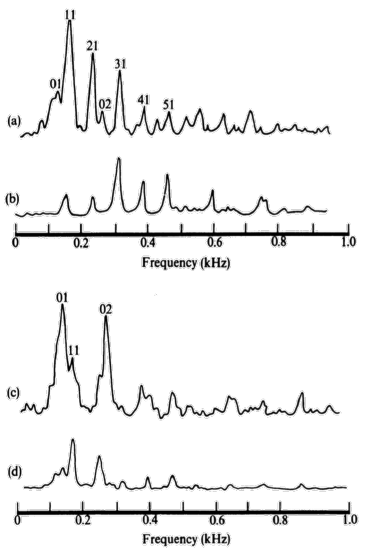
\includegraphics[height=0.3\textheight]{00_Images/08,09,10_chapter/01.png}
    \caption{Different sound spectra of a timpani}
    \label{fig:timpanisoundspectra}
\end{figure}

\section{Bass Drums}

\subsection{General Structure}

A bass drum typically mounts two membranes on opposite sides of a shell: a batter head and a resonant head. The tension relationship between these heads strongly influences timbre and partial decay times; commonly, the batter head is tuned to a higher tension than the resonant head. Bass drums are used as standalone orchestral instruments and as part of drum kits. 

\subsection{Modal Frequencies and Coupling of the Two Heads}

When the batter and resonant heads have the same tension, the coupled \((0, 1)\) behavior can be approximated by a two-mass oscillator. If \( f_0 \) denotes the frequency of either uncoupled head and \( f_a \) is a coupling frequency determined by the enclosed air stiffness and membrane masses, the normal modes occur at
\[
f_- = f_0
\]
and
\[
f_+ = \sqrt{ f_0^2 + 2 f_a^2 }
\]
In practice, the same mode index pair can appear at more than one frequency due to coupling effects, as illustrated by cases where a \((0, 1)\) pair is observed near both \SI{44}{\hertz} and \SI{104}{\hertz}. 

\subsection{Tension Relationship and Decay Rates}

When the batter head is overtensioned relative to the resonant head, modal decay rates are typically in the range \SIrange{3}{9}{\decibel\per\second}. In this configuration, removing the resonant head does not substantially change these decay rates. When both heads are tuned to the same tension, modes tend to decay faster, with rates around \SIrange{6}{11}{\decibel\per\second}. For lower-frequency modes with long wavelengths, decay also depends on interaction with the surrounding acoustic environment.

\subsection{Transient Tension Increase and Pitch Fall}

Immediately after a strong impact, the average membrane surface tension increases, producing an instantaneous rise in modal frequencies. As the tension relaxes back to its nominal value, modal frequencies decrease. This mechanism contributes to the characteristic pitch fall that can be heard in long-resonating bass drums struck with high force. 

\section{Snare Drums}

\subsection{General Structure and Materials}

A snare drum mounts two heads on the two sides of the shell. A set of snares (wires) is tightened against the resonant head, producing the characteristic buzzing component of the sound. Shells are commonly made of wood, such as maple, birch, or bubinga, or of metals, such as copper, brass, and steel. Marching-band snare drums differ markedly from typical drum-kit snares in construction and use.

\subsection{Lower-Mode Coupling as a Two-Mass Model}

The coupling of the first low-order modes of the two drumheads can be represented by a two-mass model in which the heads have different effective masses and spring constants. The coupled system is described by:

\begin{itemize}
    \item batter head mass \( m_b \) and spring constant \( K_b \),
    \item resonant head mass \( m_s \) and spring constant \( K_s \),
    \item coupling spring \( K_c \) associated with the enclosed air volume.
\end{itemize}

Introducing the angular-frequency parameters
\[
\omega_b^2 = \frac{K_b}{m_b} , \quad \omega_s^2 = \frac{K_s}{m_s} , \quad \omega_{cb}^2 = \frac{K_c}{m_b} , \quad \omega_{cs}^2 = \frac{K_c}{m_s}
\]
the two normal-mode angular frequencies satisfy
\[
\omega_{\pm}^2 = \frac{1}{2}\left( \omega_b^2 + \omega_s^2 + \omega_{cb}^2 + \omega_{cs}^2 \pm \sqrt{\left( \omega_b^2 + \omega_{cb}^2 - \omega_s^2 - \omega_{cs}^2 \right)^2 + 4 \omega_{cb}^2 \omega_{cs}^2} \right)
\]
These two normal modes combine on the two heads in a similar way and can be associated with the \((0, 1)\) behavior of the individual membranes. 

\subsection{Shell Modes and Possible Interactions}

The shell itself exhibits structural modal shapes even when drumheads are not mounted. These shell vibrations can contribute additional resonant features and participate in coupling mechanisms when heads are present, especially through the mechanical boundary conditions at the rims.

\begin{figure}[!htb]
    \centering
    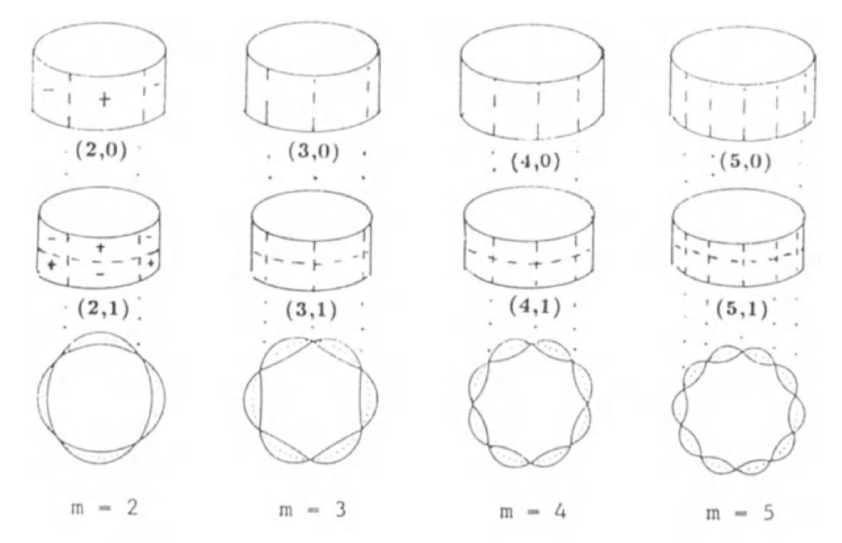
\includegraphics[width=0.7\linewidth]{00_Images/08,09,10_chapter/02.png}
    \caption{Snare shell modal shapes}
    \label{fig:snaremodal}
\end{figure}

\subsection{Snares Action}

Snares detach from the vibrating head and strike back against it, injecting high-frequency components into both the head motion and the snares themselves. Snare velocity depends on stroke intensity and snare tension, while low-tension snares produce greater damping of the resonant head. 

\section{Tom Toms}

Tom toms are used both as standalone instruments and as components of drum kits. Rack toms are typically mounted through suspension systems, while floor toms use legs to elevate the shell from the floor. The resonant head may be omitted in some designs, and open (single-head) toms tend to exhibit a clearer pitch character.

\section{Drumhead Types}

A wide variety of drumheads exists, and several construction features are commonly varied:

\begin{itemize}
    \item central reinforcement such as a power-dot,
    \item number of plies, including single-ply and double-ply heads,
    \item hydraulic film layers within double-ply heads,
    \item reinforcement rings,
    \item clear versus coated surfaces.
\end{itemize}

All these characteristics influence drum tone, harmonicity, and decay time by modifying the local mass, stiffness, and damping distributions on the membrane.

\section{Indian Drums}

\subsection{Tabla}

Tabla is typically played together with a larger bass companion instrument, often referred to as banya. A strong harmonic character is obtained by applying a central reinforcement to the drumhead. The head is commonly described as a multi-ply animal skin, and the central reinforcement can be produced by a paste made from boiled rice mixed with heavy metal particles. Tuning is achieved through the positioning of wooden cylinders within the leather thongs that tighten the head.

\paragraph{Remark on demonstrations} Short sound demonstrations are often used to emphasize the distinct tonal outcome produced by the reinforced central region.

\subsection{Mrudanga}

Mrudanga is a two-headed drum originating from southern India. The smaller head emulates the tabla-like behavior, while the larger head provides a bass response analogous to the banya. Similar drumhead treatments are applied on both sides to shape harmonicity. 

\subsection{Common Characteristics of Reinforced Indian Drumheads}

Reinforced Indian drumheads exhibit strong harmonic content, with the first four overtones often aligned as harmonics of the fundamental. Harmonic components can arise from combinations of several modes with very close frequencies. The harmonicity properties are attributed to the head reinforcement, which can be realized through many thin stacked layers, sometimes exceeding 100 layers; increasing the number of layers tends to increase harmonicity.
